% Maintenance records and reports
\chapter{registros e relat�rios de manuten��o}
A implementa��o das mudan�as requisitadas esta sendo realizada.

% Describe how information will be collected and provided
\section{Descreva como as informa��es ser�o coletadas e fornecidas}
As informa��es ser�o coletadas manualmente pelo respons�vel pela manuten��o.

% Lists of requests for assistance, modification requests, or problem reports
\section{Listas de pedidos de assist�ncia, solicita��es de modifica��o ou relat�rios de problemas}

\begin{figure}[!hb]
	\centering
	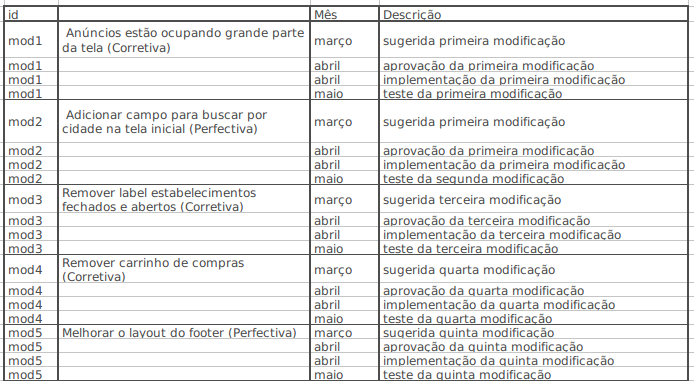
\includegraphics[width=0.7\linewidth]{historico_modificacoes_00}
	\caption{}
	\label{fig:historicomodificacoes00}
\end{figure}

\begin{figure}[!hb]
	\centering
	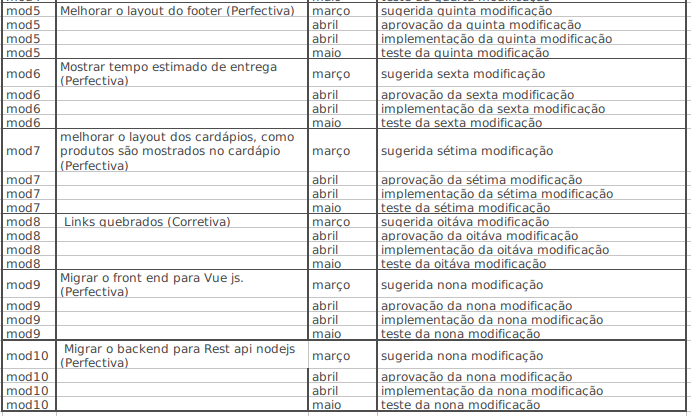
\includegraphics[width=0.7\linewidth]{historico_modificacoes_01}
	\caption{}
	\label{fig:historicomodificacoes01}
\end{figure}


% Status of requests by categories 
\section{Status dos pedidos por categorias}

% Priorities of requests 
\section{Prioridades dos pedidos}

	C�digo do �tem e sua prioridade.

\begin{enumerate}[label=(\roman*)]
	
	\item mod1 Alta
	\item mod2 Alta
	\item mod3 M�dia
	\item mod4 M�dia
	\item mod5 M�dia
	\item mod6 Baixa
	\item mod7 Baixa
	\item mod8 Baixa
	\item mod9 Baixa
\end{enumerate}

% Measurement data to be collected on maintenance activities
\section{Dados de medi��o a serem coletados em atividades de manuten��o}